\documentclass[10pt,a4paper,twocolumn]{article}
\usepackage[T1]{fontenc}
\usepackage{url}
\usepackage[spanish]{babel}
\usepackage{amsmath}
\usepackage{amssymb}
\usepackage{caption}
\usepackage{subcaption}
\usepackage{siunitx}
\usepackage{listings}
\usepackage{graphicx}
\usepackage{makecell}


\title{Métodos numéricos para la solución de problemas de optimización}
\author{Jackson Vera Pineda}
\date{}

\begin{document}
	




	\maketitle
	\selectlanguage{spanish}
	
	
	\section{Introducción}
	
	John von Neumann, uno de los mas grandes matemáticos dek siglo XX, expresó: \emph{"la optimización es el arte de obtener lo mejor de lo disponible"} \cite{von2018mathematical}. En esta frase se captura la esencia de un campo que ha demostrado ser crucial para resolver problemas complejos y de diversas disciplinas. En la actualidad, los algoritmos de optimización permiten abordar tareas intratables, obteniendo soluciones (o aproximaciónes de estas), incluso en espacios de búsqueda vastos y multidimensionales.
	
	En este trabajo, nos centramos en la aplicación de algoritmos de optimización para resolver problemas en los que la función objetivo presenta una estructura compleja, como el siguiente caso:
	\begin{equation}
		f(x) = - \frac{1}{D} \sum_{i=1}^D x_i sin(\sqrt{|x_i|})
	\end{equation}
	donde $x_i$ son las variables de decisión y $D$ es la dimensión del espacio en que opera el algoritmo. Esta función posee mínimos locales multiples y discontinuidades en el comportamiento de sus derivadas, lo que la convierte en un desafío para técnicas tradicionales de optimización.
	
	Para abordar el problema (1) exploramos y comparamos el desempeño de diversos algoritmos de optimización incluyendo \textbf{Recocido Simulado}, \textbf{Evolución Diferencial} y el método \textbf{L-BFGS-B} (Cuasi-Newton). Estos métodos se seleccionaron por su eficacia reconocida en escenarios con diferentes características geométricas y sus capacidades para manejar restricciones en las variables de decisión, como límites en los valores de \(x_i\) en el rango de \([-500, 500]\).
	
	Históricamente, la búsqueda de soluciones óptimas en sistemas complejos ha evolucionado desde enfoques analíticos hacia métodos computacionales. Un ejemplo destacado es el desarrollo del algoritmo de recocido simulado en los años 80, inspirado en los procesos de enfriamiento lento de materiales. La simulación de este fenómeno natural permitió resolver problemas combinatorios extremadamente difíciles \cite{kirkpatrick1983optimization}. De manera similar, el desarrollo de técnicas como evolución diferencial en la década de los 90 proporcionó herramientas poderosas para encontrar soluciones en espacios de búsqueda no diferenciables y de alta dimensionalidad \cite{storn1997differential}.
	
	A lo largo de este trabajo, medimos y comparamos el costo computacional de los distintos métodos a medida que la dimensionalidad del problema crece. Nuestro objetivo es identificar qué algoritmo ofrece un balance óptimo entre precisión y costo temporal, permitiendo así una mejor toma de decisiones en problemas con restricciones complejas y funciones objetivo difíciles.
	
	\section{Desarrollo}
		
		
		
		
	
		\subsection{Función objetivo}
		
			En el presente, se toma la función número 128 propuesta en el estudio de literatura sobre funciones de referencia para problemas de optimización global \cite{jamil2013literature}, descrita en el sección anterior. En el estudio proveen datos de interés sobre (1), como mínimo $f(x^*) = -418,983$ situado en $x^* = \pm [ \pi (0.5 + k)]^2$ que usaremos como puntos de referencia para analizar el desempeño de los algoritmos empleados.
			
			Dicha función es una suma de términos que involucran relaciones no lineales (raíces cuadradas y senos), de ahí que presente comportamientos peculiares y múltiples mínimos locales como puede observarse en la figura \ref{fig:1} para valores de $D=1,2$. 
		
			\begin{figure}[htb!]
					\centering
			\begin{subfigure}{.75\linewidth}
				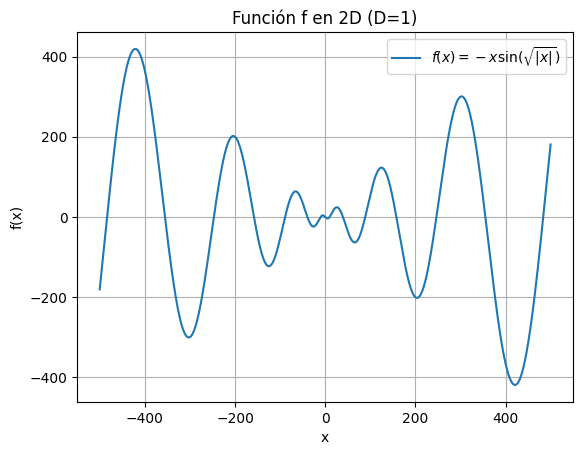
\includegraphics[height=.95\linewidth, width=.95\linewidth]{assets/f_2d}
				\caption{}
				\label{fig:1a}
			\end{subfigure}
			\begin{subfigure}{.75\linewidth}
				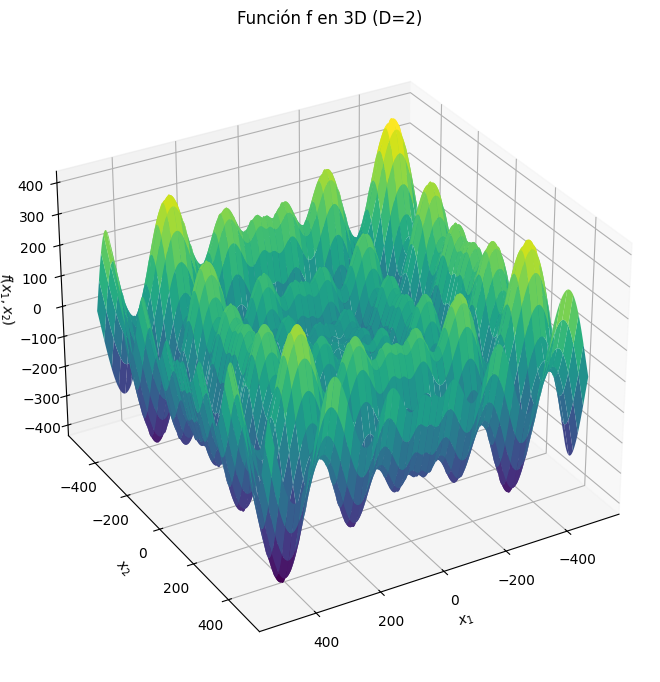
\includegraphics[height=.95\linewidth, width=.95\linewidth]{assets/f_3d}
				\caption{}
				\label{fig:1b}
			\end{subfigure}
			\caption{Representación gráfica de la función $f$ (1) para varios valores de D.}
			\label{fig:1}
		\end{figure}
	
		\subsection{Métodos}
		
			Teniendo en cuenta las carácteristicas de la función y los algoritmos encontrados en bibliografías clásicas, se utilizan los siguientes métodos para la resolución de $f$. Nótese que estos algoritmos son dependendientes de la dimensión del problema, lo cual en algunos casos es un factor crítico en su rendimiento. En la figura \ref*{table:1} se presenta una tabla con un resumen comparativo de los algoritmos teniendo en cuenta su documentación, sirviendo de punto de partida, para su posterior análisis empírico.
			
			\subsubsection{Recocido Simulado}
				Es un algoritmo de optimización global que simula el proceso de enfriamiento de los metales. Requiere un número grande de evaluaciones de la función objetivo y explora el espacio de búsqueda con cierto grado de aleatoriedad, permitiendo escapar de mínimos locales; fue introducido por Kirkpatrick et al. en 1983 \cite{kirkpatrick1983optimization} y es un enfoque bien conocido para evitar mínimos locales en problemas complejos. Su eficiencia temporal depende de la configuración del enfriamiento y del tamaño del espacio de búsqueda.
				
				Costo asintótico: Aproximadamente $ O(k \cdot D) $, donde $ k $ es el número de iteraciones, que a menudo debe ser grande para un espacio de búsqueda amplio.
				
				
			\subsubsection{Evolución Diferencial}
				Es un algoritmo de optimización global basado en la evolución de una población de soluciones candidatas, utilizando mutaciones y recombinaciones. Similar a Simulated Annealing, pero basado en métodos evolutivos; fue introducida por Storn y Price en 1997 \cite{storn1997differential}. Se ha reconocido como un método robusto para la optimización global, particularmente en problemas de alta dimensión y no diferenciables. La eficiencia temporal depende del número de evaluaciones de la función objetivo y del tamaño de la población.
				
				Costo asintótico: Aproximadamente $O(P \cdot k \cdot D) $, donde $ P $ es el tamaño de la población y $k$ es el número de iteraciones.
				
				
			\subsubsection{L-BFGS-B}
			 Es un método cuasi-Newton que utiliza una aproximación a la matriz Hessiana (segunda derivada) de la función objetivo en lugar de calcularla directamente, con uso limitado de memoria, lo que puede ser computacionalmente más eficiente que el método de Newton. Este algoritmo es especialmente útil para problemas grandes y maneja restricciones de caja de manera natural. Fue desarrollado por Byrd et al. en 1995 \cite{byrd1995limited}. 
			 
			 Costo asintótico: Aproximadamente $O(n \cdot m \cdot D)$, donde $n$ es el número de iteraciones y $m$ el número de pares de vectores almacenados (generalmente pequeño).
			 
		
		
		\begin{figure*}[ht!]%
			\begin{center}
				\begin{tabular}{lcccc}
					\hline
					\multicolumn{1}{c}{\textbf{Algoritmo}} & \multicolumn{1}{c}{\makecell{\textbf{Costo Asintótico} \\ \textbf{Aproximado}}} & \multicolumn{1}{c}{\makecell{\textbf{Comportamiento para} \\ \textbf{Dimensiones Grandes ($D$)}}} & \multicolumn{1}{c}{\makecell{\textbf{Optimización} \\ \textbf{Global}}} & \multicolumn{1}{c}{\makecell{\textbf{Optimización} \\ \textbf{Local}}}\\
					\hline
					Recocido Simulado  & $O(k \cdot D)$ & Aumenta rápidamente con $ D $& Sí & No \\ 
					Evolución Diferencial & $O(P \cdot k \cdot D)$ & Escala mal con $D$ & Sí & No \\
					L-BFGS-B & $O(n \cdot m \cdot D)$ & Muy eficiente para $D$ grande & No & Sí \\		  		
					\hline
				\end{tabular}
				\caption{Resumen comparativo de los algoritmos empleados.\label{table:1}}
			\end{center}
		\end{figure*}
			 
			
	\subsection{Metodología}
		Para comparar el desempeño de cada método en nuestra función, se tuvieron en cuenta el tiempo de ejecución de cada uno, la evaluación mínima obtenida, y el vector de dicha evaluación para valores de $1 \leq D \le 29$. Para cada valor de $D$, por cada algoritmo utilizado se simularon 30 ejecuciones, estas son aproximadamente $30*30*3 = 2700$ ejecuciones. De esta muestra se toma la media del tiempo por cada método y valor de dimensión, así como mejor mínimo encontrado, y punto en el que se alcanza.
		
		En la figura \ref{fig:2} se puede observar el coste temporal de los métodos, nótese como a partir de $D=10$ explota la curva que describe el rendimiento del algoritmo Evolución Diferencial, mostrando su mala escalabilidad. Nótese además el buen desempeño de Recocido Simulado (Simulated Annealing) y L-BGS-B para resolver nuestra problema.
			
		\begin{figure}[htb!]
			\centering
			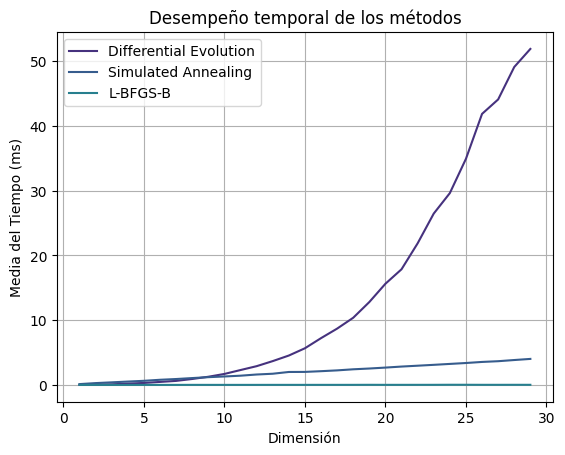
\includegraphics[height = .75\linewidth, width=.75\linewidth]{assets/time_comp}
			\caption{Comparación del tiempo medio de ejecución de cada método al aumentar la dimensión del problema.}
			\label{fig:2}
		\end{figure}
		
		Luego de observar el desempeño temporal surge, naturalmente, la pregunta ¿qué tanto se aproximan al mínimo en sus evaluaciones? Nótese en la figura \ref{fig:3} como, a pesar del buen desempeño de L-BGS-B, al aumentar la dimensión el mínimo encontado se aleja de la repuesta, mostrando su sensibilidad a mínimos locales; en cambio Recocido Simulado y Evolución Diferencial, se muestran robustos al aumento dimensional. Comportamineto similar se observa en la figura \ref{fig:4} de cuanto se alejan los puntos encontrados del punto en el cual $f$ alcanza su mínimo (en el intervalo $-500 \leq x_i \leq 500$), teniendo como medida la raíz del error cuadrático medio.
		
		\begin{figure}[htb!]
			\centering
			\begin{subfigure}{.492\linewidth}
				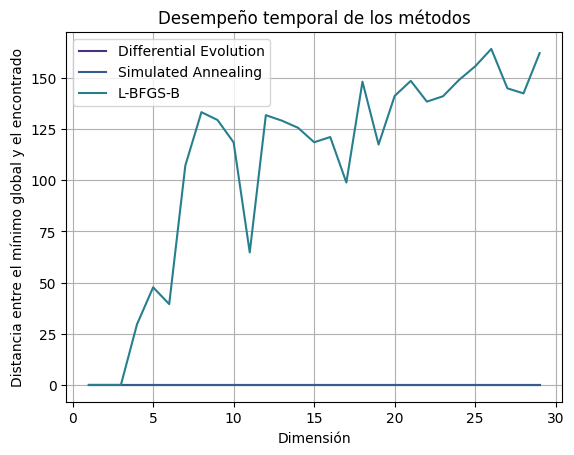
\includegraphics[height=.95\linewidth, width=.95\linewidth]{assets/ev_comp}
				\caption{}
				\label{fig:3a}
			\end{subfigure}
			\begin{subfigure}{.492\linewidth}
				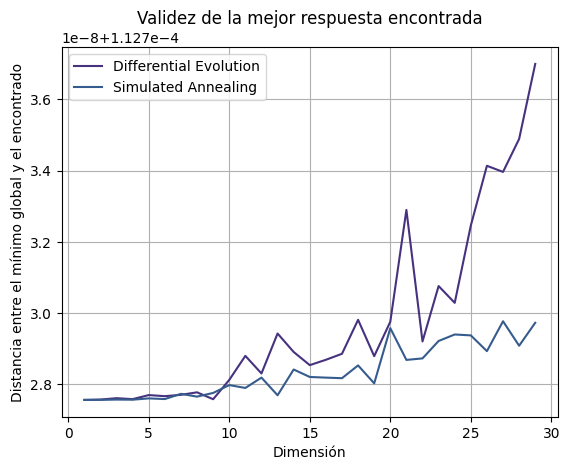
\includegraphics[height=.95\linewidth, width=.95\linewidth]{assets/ev_comp2}
				\caption{}
				\label{fig:3b}
			\end{subfigure}
			\caption{Comparación del error entre el mínimo encontrado y el mínimo global de la función $f(x^*) = -418,983$, al aumentar la dimensión del problema.}
			\label{fig:3}
		\end{figure}
		
			\begin{figure}[htb!]
			\centering
			\begin{subfigure}{.492\linewidth}
				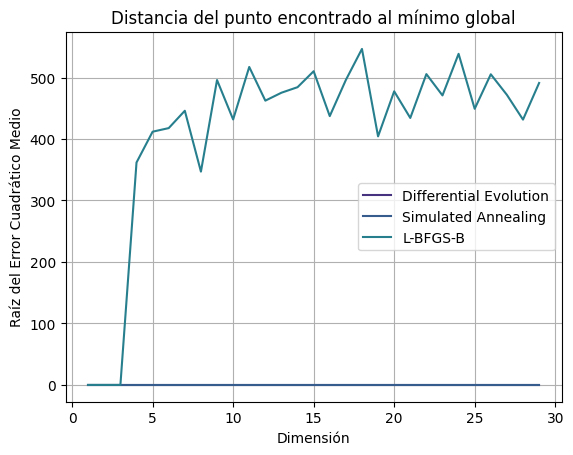
\includegraphics[height=.95\linewidth, width=.95\linewidth]{assets/rmse_comp}
				\caption{}
				\label{fig:4a}
			\end{subfigure}
			\begin{subfigure}{.492\linewidth}
				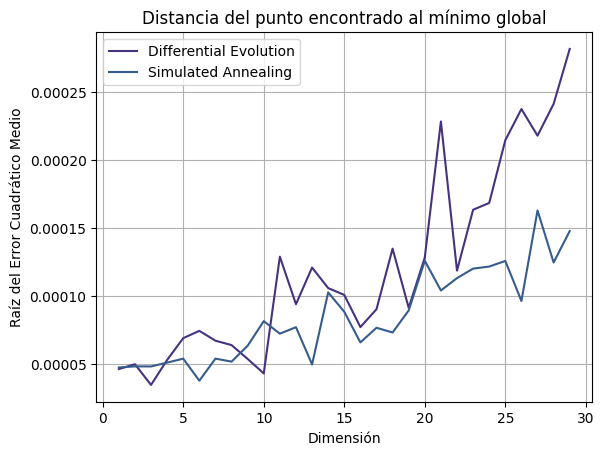
\includegraphics[height=.95\linewidth, width=.95\linewidth]{assets/rmse_comp2}
				\caption{}
				\label{fig:4b}
			\end{subfigure}
			\caption{Comparación de la raíz del error cuadrático medio entre el punto de mínimo y el punto de mínimo global de la función $x^* = [ \pi (0.5 + k)]^2$ para $k=6$, al aumentar la dimensión del problema.}
			\label{fig:4}
		\end{figure}
	
	
	\section{Conclusiones}
		Teniendo en cuenta el comportamiento de los algoritmos para el problema no lineal presentado, Recocido Simulado mostro tener un buen balance entre costo temporal y calidad de la solución, en comparación con las alternativas analizadas. Se probó lo costoso que puede llegar a ser Evolución Diferencial para problemas de alta dimencionalidad, criterio que se alinea con lo enunciado sobre este en la bibliografía, así como, aun siendo costoso mantiene resultados fiables. A diferencia de L-BFGS-B, cuya eficiencia es incomparable, sin embargo, su sensibilidad a mínimos locales juega un papel crítico en problemas con características similares a la función analizada, por lo que sus resultados deben ser validados e interpretados cuidadosamente.
	
	\bibliographystyle{plain}
	\bibliography{assets/biblo.bib}
	
\end{document}